\section{Code Design}

\subsection{Some Comments}

In designing a code in C the main object of which is to do high
performance computing, there are some inevitable tensions with
software engineering best-practice. In particular, complete
encapsulation of data in the spirit of using abstract data types
tends to cause problems of performance.

For example, encapsulation of the lattice Boltzmann distribution
$f_i$, together with appropriate ``get'' and ``set'' functions for
access when approapriate, is possible. There could then be a
complete separation of interface and implementation of the
distribution (other than that each individual $f_i$ is represented
by a \texttt{double}). However, experience suggests that
this imposes severe impediment to optimisation and hence
unacceptable performance degradation.

Schemes do exist by which one can approximate the object
oriented programming style in C, and so achieve a separation
of interface and implementation. However, this tends to put
a heavy burden on the use of \texttt{void} pointers, itself
a recipe for possible disaster. A truly object-oriented
language such as Java would be preferable.

So, for the time being, some relaxation of encapsulation is required.
Exposing a pointer to the distributions which allows them to be accessed
directly where required. This can be done merely by declaring the
necessary variables \texttt{extern}. In practice, such deviations
from encapsulation can be minimised in the lattice sector of the
code. In particlar, \texttt{extern} declarations should not be
required in \texttt{main()}, i.e., it should be able to write a
new application without worrying about details of implementation.

\subsubsection{Objects}

Somewhat more difficult is the part of the code involving
colloids, which would really favour a truly object-oriented
approach.

\subsubsection{Serial and parallel}

The design decission has been taken to support execution of the
code in both serial and parallel. The default compilation
assumes that a serial executable is required, while  MPI code
is introduced via C-preprocessor directives (\texttt{-D\_MPI\_}).


There is no shared memory inplementation at this time.


\subsection{Structural Components: \texttt{MPI\_COMM\_WORLD}}


\subsection{Coordinate System: \texttt{MPI\_CARTESIAN\_COMMUNICATOR}}


\begin{figure}
\begin{center}
%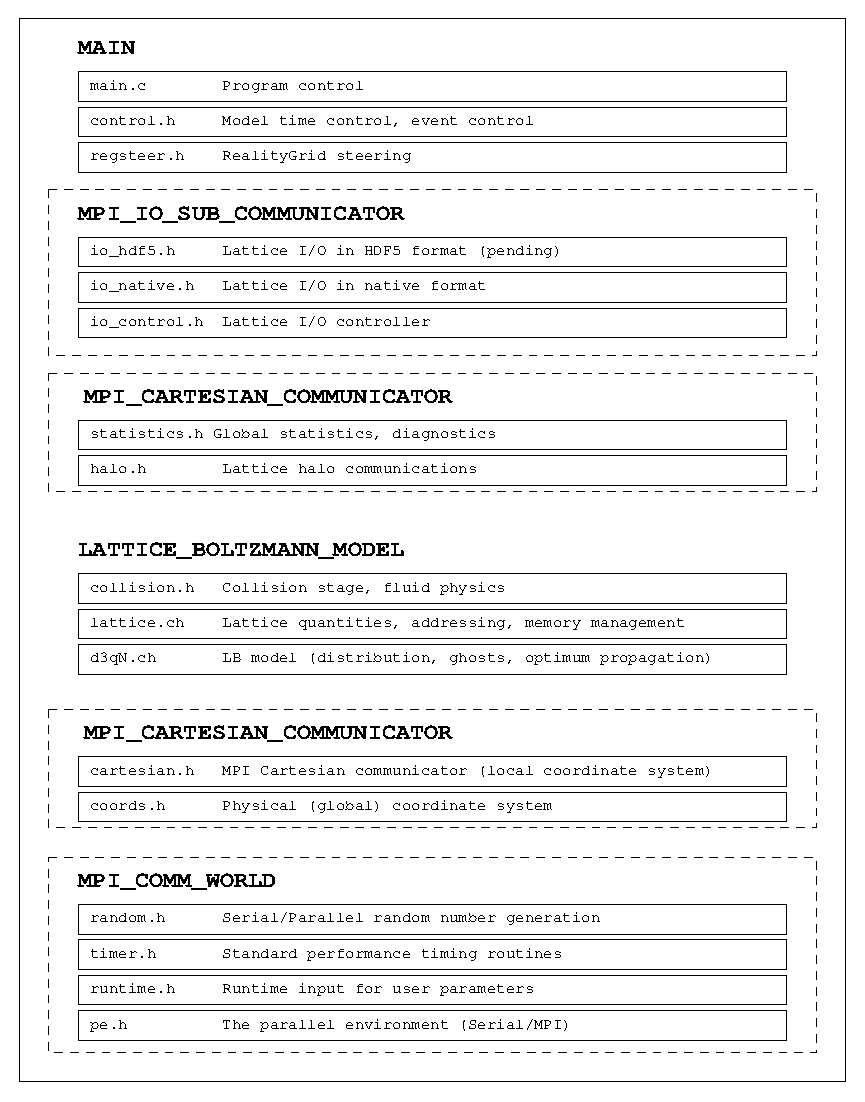
\includegraphics{xfig/sketch.eps}
\end{center}
\caption{A scheme by which different parts of the code might be
encapsulated and in such a way to allow reliable development and
testing. As this is C, will do not adopt a truly ``object'' langauge.
Broadly, different modular parts should only depend on stuff above
in the diagram. So, at the top, there is the parallel environment
where communication occurs within MPI\_COMM\_WORLD. Built on top
of this is the Cartesian Communicator responsible for halo swaps
and so forth. The LE code may have a separate Communicator again. 
(There's an argument to say the diagram should be the other way up!)}
\end{figure}

\clearpage
\vfill\pagebreak

\section{Code Implementation}

\subsection{Stuff}

\subsection{Coordinate System}

\subsubsection{The global coordinate system}

The user specifies the system size in lattice units at run time,
which sets the extent of memory which must be allocated for the
Cartesian lattice. The extent of the physical coordinate system
then reflects the lattice size directly (see Figure \ref{fig_c1}). 
Each lattice site, or node,  has coordinates corresponding to its
integer position in the system and can be thought of as being
at the centre of a control volume one lattice unit on a side.
This means that the nominal edges of the
system are offset from the lattice sites themselves by half a
lattice unit in each direction.


\begin{figure}[h]
\begin{center}
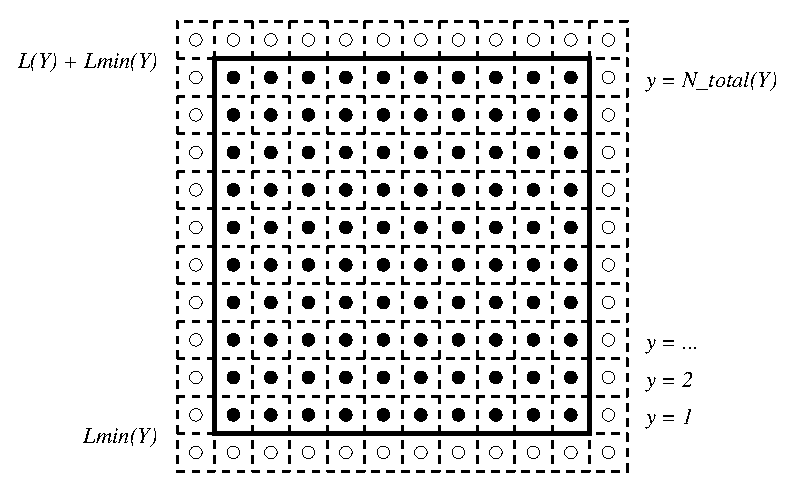
\includegraphics{xfig/fig_c1.eps}
\end{center}
\caption{The global Cartesian coordinate system reflects the choice
of lattice size; lattices sites are located at
$x=1, \ldots, x = N_{total}$ and so on in each coordinate direction
(the Figure only shows the labels in the $y-$direction for simplicity).
In the Figure, the lattice sites in the domain proper are the full
circles; halo sites, which are used to effect periodic boundary
conditions, are included as open cirles}
\label{fig_c1}
\end{figure}

For particles, the centres of which can move continuously across the
lattice, the extents of the global coordinate system are then
$L_{min} < x < L + L_{min}$ and so on.

\subsubsection{Addressing the lattice: the local coordinate system}


\subsection{Solid walls}

General solid objects which are fixed for the duration of
the simulation, such as porous media, can be defined
by assigning solid/fluid status to each lattice node. 
The links required between solid and fluid nodes can
then be identified for the given model.

\textit{Comment.} In general, a solid object will not
affect the periodic nature of the simulation. A general
solid object cannot move, i.e., the boundary velocity
must be zero.

\textit{Special case.} In the case where the solid object
represents a flat boundary wall at the edge of the system
in one or more directions, the periodicity is broken in
the corresponding directions.



%%%%%%%%%%%%%%%%%%%%%%%%%%%%%%%%%%%%%%%%%%%%%%%%%%%%%%%%%%%%%%%%%%%%%%%%%%%%%
% LE Implementation
%%%%%%%%%%%%%%%%%%%%%%%%%%%%%%%%%%%%%%%%%%%%%%%%%%%%%%%%%%%%%%%%%%%%%%%%%%%%%

\subsection{Lees Edwards Sliding Period Boundary Conditions}

\subsubsection{The LE module}

\subsubsection{Distributions crossing the LE planes}

With the planes conceptually half-way between lattice sites, the
propagation moves some of the distributions (namely, those with
$c_x = \pm1$) between different sliding blocks. While the collision
stage is unaffected, action must be taken to adjust these
distributions when the LE boundary conditions are active. This
is done in a two-stage process described by Adhikari \textit{et al.}
\cite{adhikari_desplat}, implemented between the collision and
propagation.

\textbf{a. Reprojection} The post-collision distributions with
$c_x = \pm 1$ at sites adjacent to a boundary are modified to
take account of the velocity jump $\pm u^{LE}_y$ between the sliding
blocks. In terms of the hydrodynamic moments we have:
\begin{eqnarray}
\rho &\rightarrow& \rho', \\
\rho u_\alpha &\rightarrow& (\rho u_\alpha)' \pm \rho' u^{LE}_\alpha, \\
S_{\alpha\beta} &\rightarrow&
S'_{\alpha\beta} \pm (\rho u_\alpha)' u^{LE}_\beta
\pm (\rho u_\beta)' u^{LE}_\alpha + \rho' u^{LE}_\alpha u^{LE}_\beta.
\end{eqnarray}
If we work with the changes to the moemnts, then the density is
unaffected $\delta\rho =  0$, the velocity is changed by
$\delta u_\alpha = \pm u^{LE}_\alpha$, with an analogous expression for
the change in the stress
\begin{equation}
\delta S_{\alpha\beta} =
\pm (\rho u_\alpha)' u^{LE}_\beta
\pm (\rho u_\beta)' u^{LE}_\alpha + \rho' u^{LE}_\alpha u^{LE}_\beta.
\end{equation}
We can then work out the change in the distributions by reprojecting
via Eq.\ref{eq:}, i.e.,
\begin{equation}
f_i \rightarrow f_i' + w_i \Bigg(
\frac{\rho \delta u_\alpha c_{i\alpha}}{c_s^2} +
\frac{\delta S_{\alpha\beta}Q_{i\alpha\beta}}{2c_s^4} \Bigg).
\end{equation}
A similar set of expressions are given for the order parameter
distributions in Adhikari \textit{et al.} \cite{adhikari_desplat}.

\textbf{b. Interpolation of reprojected distributions}
As the sliding blocks are displaced continuously with
$\delta y = u_y^{LE}t$, which is not in general a whole number of
lattice spacings, an interpolation is also required before
propagation can take place. Consider the situation (Fig.~\ref{fig_le2}) from
a stationary frame where the frame above has translated a small
distance to the right ($\delta y < \Delta y$). In the stationary frame
we must interpolate the ditributions with $c_x = 1$ to a
`departure point' from which the propagation will move the
distribution exactly to the appropriate lattice site in the moving
frame. Schemeatically,
\begin{equation}
f_i'(x, y + \delta y, z) = 
 (1 - \delta y) f_i^\star(x, y, z) +
\delta y f_i^\star(x, y + \Delta y, z),
\end{equation}
where $f_i'$ here represents the interpolated value and $f_i^\star$
is the reprojected post-collision quantity.

In the case where the displacement $\delta y > 1$, the relevant
lattice sites involved in the interpolation are displaced to the right
by the integral part of $\delta y$, while the relative weight given to
the two sites involves
the fractional part of $\delta y$. To take account of the periodic
boundary conditions
in the $y$-direction, all displacements are modulo $L_y$.


\begin{figure}[h]
\begin{center}
%\includegraphics{xfig/fig_le2.eps}
\end{center}
\caption{Schematic diagram showing interpolation of distributions in the
stationary plane (below) in preparation for propagation into the moving
frame (above). For a small displacement $\delta y = u^{LE} t$, the
interpolation takes place between lattice sites in the stationary frame
(green, left). Propogation from the interpolated positions (red) can
then take place into the moving frame (right).}
\label{fig_le2}
\end{figure}


In parallel, exactly the same calculation is undertaken. However,
communication is required to take account of the processor
decomposition in the $y$-direction. This requires the identification
of the two processes which hold the relevant information as a function
of displacement. 

Note that the interpolated values are stored in the appropriate lattice
site in the rest frame that ensures the normal propagation stage moves all
distributions to the correct destination in memory.

\subsubsection{Order parameter gradients}

When the order parameter gradient is computed at a given point
near the LE boundaries, the stencil may extend out of the stationary
frame. The process of interpolation is slightly different to that
for the distributions.

Here, we need to interpolate values in the moving frame to the position
which is seen by the rest frame. Figure~\ref{fig_le3} shows a five-point
stencil to calculate the gradient at the central point $(x,y,z)$ in the
rest frame. An interpolation of the $\phi$-field of the form
\begin{equation}
\phi'(x + \Delta x, y - \delta y, z) =
\delta y \phi(x + \Delta x,  y - \Delta y, z) + 
(1 - \delta y) \phi(x + \Delta x, y, z)
\end{equation}
must then take place. In practice, the interpolated values are stored
in the offset buffer. As the gradient calculation requires $\phi$
values in the halo regions, interpolated values for the buffer halo
region are also required.

\begin{figure}[h]
\begin{center}
%\includegraphics{xfig/fig_le3.eps}
\end{center}
\caption{Schematic diagram showing a five-point stencil to compute a
gradient at the central point in the stationary frame. The upper point
of the stencil is in the moving frame and so must be interpolated to
the correct position (red sites).}
\label{fig_le3}
\end{figure}

In parallel, the interpolation requires data from at most two adjacent
processes in the along-plane $y-$direction as long as the $\phi$ halo
regions are up-to-date. The rank of the processes involved is
determined by the displacement $\delta y$ as a function of time.


\subsubsection{Velocities and finite-difference fluxes}

For the finite-difference implementation, the velocity field at
the cell boundaries is required. At the planes, this means an
interpolation which takes the same form as that for
$\phi$ is needed.

In computing the advective fluxes between cells, we must then
allow for the presence of the planes. This is done by computing
separately the 'east' and 'west' face fluxes in the $x$-direction
(the flux that crosses the plane). Away from the planes, face-flux
uniqueness $f_{ijk}^e = f_{i+1jk}^w$ ensures conservation of order
parameter. However, at the planes, the non-linear conbination of
velocity field and order parameter field does not in general give
rise to consistent fluxes. In order to restore conservation, we
reconcile east and west face fluxes at the plane by taking an
average
\begin{eqnarray}
f_{ijk}^{e\star}&=&{\textstyle\frac{1}{2}}(f_{ijk}^e + f_{i+1j'k}^w),\quad 
f_{i+1j'k}^w  = \delta y f_{i+1 j-1 k}^w + (1 - \delta y) f_{i+1jk}^w,\\
f_{i+1 j k}^{w\star} &=& {\textstyle\frac{1}{2}}(f_{ij'k}^e + f_{i+1jk}^w),\quad
f_{ij'k}^e = (1 - \delta y) f_{ijk}^e + \delta y f_{ij+1k}^e.
\end{eqnarray}
In this way, we average the east face flux in the rest frame $f_{ijk}^e$
with the interpolated value of the west face flux in the moving frame
$f_{i+1j'k}^w$, and vice-versa. One can then easily show that when
integrated over the length of the plane, the average fluxes are
consistent, i.e.,
\begin{equation}
\sum_j (f_{ijk}^{e\star} - f_{i+1jk}^{w\star}) = 0 \quad\forall k,
\end{equation}
thus ensuring order parameter conservation.

A similar correction is required when computing the force on the fluid
directly via the divergence of the thermodynamic stress
$F_\alpha = \nabla_\beta P_{\alpha\beta}^{th}$. This is implementated
by computing fluxes of momentum at cell faces in each direction, and
then taking the divergence to compute the force. At the planes, an
averaging procedure is again used to ensure conservation of momentum.

%%%%%%%%%%%%%%%%%%%%%%%%%%%%%%%%%%%%%%%%%%%%%%%%%%%%%%%%%%%%%%%%%%%%%%%%%%%%%
% End LE implementation
%%%%%%%%%%%%%%%%%%%%%%%%%%%%%%%%%%%%%%%%%%%%%%%%%%%%%%%%%%%%%%%%%%%%%%%%%%%%%


\clearpage
\vfill\pagebreak

\section{Code Interface}

\subsection{The Parallel Environment}

\texttt{\#include ``pe.h''}

As the code is to be available in both serial and parallel versions,
it is desirable to abstract the basic environment to some extent.
The parallel environment is intended to support MPI communication
within \texttt{MPI\_COMM\_WORLD}, or fall back to a minimally
consistent picture in serial (i.e., rank zero is the single process).

\texttt{void pe\_init(int argc, char ** argv)}\\
Responsible for initialisation of MPI, and hence must be first
execuatable statement. The arguments are those to \texttt{main}
which will be passed through to \texttt{MPI\_Init()}.

\texttt{int pe\_rank(void)}\\
Returns the process rank in \texttt{MPI\_COMM\_WORLD}, or 0 in
serial.

\texttt{int pe\_size(void)}\\
Returns the number of processes in \texttt{MPI\_COMM\_WORLD}, or
1 in serial.

\texttt{void pe\_finalise(void)}\\
Responsible for \texttt{MPI\_Finalize()}, and must be the last
executable statement.

\texttt{void info(const char * fmt, ...)}\\
Behaves like \texttt{printf}, but only produces output on the
root process.

\texttt{void verbose(const char * fmt, ...)}\\
Behaves as \texttt{printf} and reports the rank of the
calling process in \texttt{MPI\_COMM\_WORLD}.

\texttt{void fatal(const char * fmt, ...)}\\
Prints an error message and identifies
the rank of the calling process before terminating the program.


\subsection{Run Time Input}

\texttt{\#include ``runtime.h''}

The ability to set a wide range of parameters at run time is
very convenient, and is supported via an input file in which the
user specifies parameters as key value pairs. The code maintains
a list of key value pairs from which the user can retrieve the
appropriate values for given keys.


\texttt{void RUN\_read\_input\_file(const char * input\_file\_name)}\\
This reads the named input file and sets up the list of keys.

\texttt{int RUN\_get\_double\_parameter(const char *key, double * value)}\\
Set the \texttt{value} associated with \texttt{key}, if present. The number
of key matches found is returned (i.e., 0 or 1).

\texttt{int RUN\_get\_int\_parameter(const char * key, int * value)}\\
Set the \texttt{value} associated with \texttt{key}, if present. The
number of key matches is returned.

\texttt{int  RUN\_get\_string\_parameter(const char * key, char * value)}\\
Set \texttt{value} to the string assocaited with \texttt{key}, if
present. Returns the number of key matches found.

\texttt{int  RUN\_get\_int\_parameter\_vector(const char * key, int v[])}\\
If \texttt{key} is present, set the associated 3-vector of integers.
Returns the number of key matches found. 

\texttt{int  RUN\_get\_double\_parameter\_vector(const char * key,
double v[])}\\
If \texttt{key} is present, set the associated 3-vector of doubles.
Returns the number of key matches found.

\textit{Comment:} We probably need a function to report unused keys, so
the user can be alerted if a key has unexpectedly been ignored.


\subsection{Random Number Generators}

\texttt{\#include ``ran.h''}

Note that the random number generation in parallel is
decomposition dependent.

\texttt{void rand\_init(void)}\\
Responsible for initialising RNG state.

\texttt{double rand\_serial\_uniform(void)}\\
Return a single variate uniformly distributed on $[0,1]$ from
the serial generator.

\texttt{double rand\_serial\_gaussian(void)}\\
Return a single variate with Gaussian distribution about zero
and having unit variance from the serial generator.

\textit{double rand\_parallel\_uniform(void)}\\
Return a single variate uniformly distributed on $[0,1]$
from the serial generator.

\texttt{double rand\_parallel\_gaussian(void)}\\
Return a single variate with Gaussian distribution about zero
and having unit variance from the parallel generator.

\textit{Comment:} The serial generator will produce the
same sequence on any MPI process, while the parallel generator
will produce different sequences. The latter is intended for
generating, specifically, fluctuations, where the need for
decomposition-independance is questionable.



\subsection{Timers}

\texttt{\#include ``timer.h''}

Performance figures require timing for different sections
of the code. The code provides a set of routines to time
standard and user-defined sections of code. Timers are
started and stopped by call to the appropriate routines.

\texttt{TIMER\_init()}\\
This initialises all the timers to zero (e.g., at the start of
the program).

\texttt{TIMER\_start(const int t\_id)}\\
Start the given timer.

\texttt{TIMER\_stop(const int t\_id)}\\
Stop the given timer.

\texttt{TIMER\_statistics(void)}\\
Prints the current state of all the active timers to standard
output on the root process in a digestible form. In serial,
the minimum, maximum, and mean time for each timer is reported
in seconds (based on the number of start/stop cycles). In
parallel, the same figures are computed on each process and the
result of the corresponding \texttt{MPI\_Reduce()} operation is
printed on the root process.

The code provides a number of timers which would time standard
parts of the code, e.g., \texttt{t\_id = TIMER\_TOTAL} for the
total execution time, and a number of spare timers for users to
use at will.


\textit{Comment:}
No intra-run variance (i.e., between time steps) is provided, as the
calculation required is considerably more complex to generalise, and
requires memory proportional to the number of time steps used.


\textit{Comment:}
Two macros, \texttt{TIMER\_START()} and \texttt{TIMER\_STOP()} are
provided to insert calls to the above functions for optional timing
of performance-sensitive regions
of the code in conjunction with the preprocessor flag
\texttt{-D\_TIMING\_MACRO\_ON\_}.


\subsection{Model Time Control}

This provides time step control, event frequency (?)

\texttt{void init\_control(void)}\\
Initialise time controls.

\texttt{int get\_step(void)}\\
Return the current model time step.

\texttt{int next\_step(void)}\\
Increments the current time step. Returns number of steps left
to run (i.e., 0 when finished).



\subsection{Coordinate System}

\texttt{\#include ``coords.h''}

A three-dimensional Cartesian coordinate system is used throughout,
with the exact system size usually chosen by the user at run time.
The symbolic constants \texttt{X}, \texttt{Y}, and \texttt{Z} are
used to identify the coordinate directions.

This also provides access to the MPI Cartesian Communicator which
is responsible for most communication in the model.

\texttt{int N\_total(const int dim)}\\
Returns the total number of lattice sites in the given Cartesian direction.

\texttt{double L(const int dim)}\\
Returns the length of the system in the given Cartesian direction
(which is the same as the number of lattice sites).

\texttt{double Lmin(const int dim)}\\
Returns coordinate position of left-hand edge of system in given
Cartesian direction.

\texttt{int is\_periodic(const int dim)}\\
Returns 1 if given Cartesian direction is periodic, else 0.

\texttt{void cart\_init(void)}\\
Responsible for setting up the Cartesian decomposition.

\texttt{int cart\_rank(void)}\\
Returns rank in the Cartesian communicator.

\texttt{MPI\_Comm cart\_comm(void)}\\
Returns the MPI Communicator handle for the Cartesian communicator.

\texttt{int cart\_size(const int dim)}\\
Returns the size of the Cartesian communicator grid in the given
coordinate direcxtion.

\texttt{int cart\_coord(const int dim)}\\
Returns the coordinate of the current process in the Cartesian
Communicator.

\texttt{int cart\_neigh(const int dir, const int dim)}\\
Returns the rank of the neighbouring process in the
Cartesian communicator.


\subsection{Colloids}

\texttt{\#include ``colloids.h''}

These functions provide the basic interface for use
of colloidal particles in the code.

\subsubsection{Colloid structure}

The basic colloid struct is defined ...
 

\subsubsection{Colloid interface}

\texttt{void colloids\_init(void)}\\
Call once for initialisation. This initialises the cell list,
so the coordinate system must be initialised via a call to
\texttt{coords\_init()} first.

\texttt{void colloids\_finish(void)}\\
Call once for finalisation. Frees all colloid-related memory.

\texttt{Colloid * allocate\_colloid(void)}\\
Returns a pointer to a newly allocated \texttt{Colloid} object
or fails gracefully.

\texttt{void free\_colloid(Colloid * p\_colloid)}\\
Deallocates all memory associated with \texttt{p\_colloid} or
fails gracefully.

\texttt{struct c\_link allocate\_boundary\_link(void)}\\
Returns a pointer to a newly allocated colloid boundary
link or fails gracefully.

\texttt{void free\_boundary\_link(struct c\_link *)}\\
Deallocates memory associated with a link or fails gracefully.

\texttt{void colloids\_memory\_report(void)}\\
The module keeps track of how much memory has been allocated in
total for colloids and boundary links. This reports the current
usage.

\texttt{get\_Ncell\_total()}\\

\texttt{get\_Ncell\_local()}\\

\texttt{Colloid * cell\_get\_colloid(int i, int j, int k)}\\
This returns a pointer to the Colloid at the head of the list at
cell list location (i, j, k) or \texttt{NULL} if there is none.

\texttt{void cell\_insert(Colloid * p\_colloid)}\\
This inserts a colloid at the head of the appropriate list
depending upon its position. This is the only way a colloid
can be added to the list.

\texttt{update\_cells(void)}\\
Performs the update of the cell list in response to updated
particle positions.

\texttt{IVector cell\_coords(FVector r)}\\




\subsection{Speculation}

\subsection{The Free Energy}

It is imagined that a single file will encapsulate all the details
of a given free energy. The interface for different choices of
free energy should be the same.


\texttt{FE\_init()}

Responsible for querying the runtime input key value pair list to
find appropriate user parameters for the free energy, or
falling back to default values.


\texttt{double FE\_get\_sigma()}

Return the surface tension. There should be a similar routine
for the interfacial thickness.

\texttt{double FE\_get\_mu(const type location)}

Return the chemical potential at the single lattice
node \texttt{location}.

\textit{Comment:} The computation of quantities such as the chemical
potential will a) affect performance and b) require halo values of
the order parameter (depending on the highest derivative
in the order parameter present). Performance here should be the
first consideration, so this needs to be handled with care.


\texttt{double pchem[ND][ND] FE\_get\_pchem(const type location)}

Return the chemical stress ${\cal P}_{\alpha\beta}$ at the
given location.

\textit{Comment:} This is an $nd \times nd$ matrix, where $nd$ is
the number of dimensions. If we are to provide explicit support for
D2Q9, \texttt{ND} will be 2, otherwise 3.


\clearpage
\vfill\pagebreak


\section{Implementation Notes}

\subsection{Serial Version}

\subsection{Efficiently Scaling Parallel Computing}

We should be thinking about the 100,000 processor regime, and
correspondingly large system sizes. To avoid embarrassment in this regime,
some issues which don't usually arise are relevant, for example:

\begin{enumerate}
\item
Large integer quantities such as
\begin{verbatim}
   N_total.x*N_total.y*N_total.z
\end{verbatim}
are likely to cause integer overflow (if default integers are 4 byte).
\item
Local data structures whose size is proportional
to the number of processors are contraindicated, e.g.,
anything like
\begin{verbatim}
p = (foo *) malloc(nprocs*sizeof(foo));
\end{verbatim}
is to be avoided. At the moment, we are in good shape on this
(apart from some functions in \texttt{misc.c}).
\item
I/O is likely become a very important issue, so may need to think
more about this.
\item
We should probably introduce a standard set of benchmarks which can
be scaled up in some systematic way, so that we can keep track of
performance over time.

\end{enumerate}


